documentclass[english]{article}

\usepackage{url}
\usepackage{tabularx}

\usepackage[utf8]{inputenc}
\usepackage[T1]{fontenc}
\usepackage{tikz}
\usepackage{babel,listings}
\tikzstyle{startstop} = [rectangle, rounded corners, minimum width=2.25cm, minimum height =1cm, text centered, draw=black,text width = 2cm]
\tikzstyle{clean} = [minimum width=1.5cm, minimum height =1cm, text centered,text width = 3cm]
\tikzstyle{arrow} = [thick,->,>=stealth]
\usepackage{ebgaramond}
\linespread{1.05}

% Adjust the height of lcmtt to match EBGaramond.
\makeatletter
\DeclareFontFamily{T1}{lcmtt}{\hyphenchar\font\m@ne}
\makeatother
\renewcommand*\ttdefault{lcmtt}
\DeclareFontShape{T1}{lcmtt}{m}{n}{%
  <13.82><16.59><11.2><23.89><28.66><34.4><41.28>%
  ecltt8}{}

% Fix EBGaramond's itemize behavior. http://tex.stackexchange.com/a/135796
\normalfont
  \makeatletter
  \input{TS1EBGaramond-LF.fd}
  \input{TS1EBGaramond-OsF.fd}
  \makeatother
  \DeclareFontShape{TS1}{EBGaramond-OsF}{m}{sl}{ <-> ssub * EBGaramond-OsF/m/it }{}
  \DeclareFontShape{TS1}{EBGaramond-OsF}{b}{n}{ <-> ssub * EBGaramond-OsF/m/n }{}
  \DeclareFontShape{TS1}{EBGaramond-OsF}{b}{it}{ <-> ssub * EBGaramond-OsF/m/it }{}
  \DeclareFontShape{TS1}{EBGaramond-OsF}{b}{sl}{ <-> ssub * EBGaramond-OsF/m/it }{}
  \DeclareFontShape{TS1}{EBGaramond-OsF}{bx}{n}{ <-> ssub * EBGaramond-OsF/m/n }{}
  \DeclareFontShape{TS1}{EBGaramond-OsF}{bx}{it}{ <-> ssub * EBGaramond-OsF/m/it }{}
  \DeclareFontShape{TS1}{EBGaramond-OsF}{bx}{sl}{ <-> ssub * EBGaramond-OsF/m/it }{}

\newcommand{\optionstable}[1]{
    \vspace{1.05em}
    \noindent
    \begin{tabularx}{\textwidth}{ c || c | X }
    Name & Type & Description \\
    \hline
    #1
    \end{tabularx}
    \vspace{1.05em}
}

\usepackage{graphicx}
\usepackage{fancyhdr}
\usepackage{multicol}
\usepackage{pdfpages}
\usepackage[colorlinks=true, linkcolor=black, urlcolor=cyan]{hyperref}

\begin{document}

\begin{titlepage}
\begin{center}
\includegraphics[height=4cm]{images/Standard_CUAUV.jpg}\\[0.2cm]
\textsl{\huge Cornell University} \\[0.05cm]
\textsl{\huge Autonomous Underwater Vehicle}\\[0.5cm]
{\huge Spring 2015}\\[0.2cm]
\rule{\linewidth}{0.5mm}\\[0.2cm]
{\Huge Creating a Commandline Cave}
\rule{\linewidth}{0.5mm}\\[0.4cm]


\emph{\huge Technical Report}\\[0.5cm]
\textsl{\large Page Bowers} \\[0.05cm]
\vfill{\today}
\end{center}
\end{titlepage}

% set up header and footer
\pdfpagewidth 8.5in
\pdfpageheight 11in

\pagestyle{fancy}
\fancyhf{}
\setlength{\headheight}{30pt}
\renewcommand{\headrulewidth}{0.4pt}
\renewcommand{\footrulewidth}{0.4pt}

\lhead{\includegraphics[height=8mm]{images/Standard_CUAUV.jpg}}
\rhead{\Large Lib-Cave}
\rfoot{Spring 2015}
\cfoot{\thepage}

% Table of contents
\tableofcontents
\pagebreak

\part{Introduction} % write to give an overview of what cave is

CAVE, or the Automated Vision Evaluator, was originally designed to help individuals test vision algorithms on video footage that was recorded during pool tests and competition.  The purpose of the system is to improve vision tuning by providing feedback with regards to the accuracy of the algorithm on frames that have been tagged.  The improvements to allow CAVE to be run from the commandline will help the user reduce the unnecessary steps the user is required to perform in order to test while using the GUI.  The commandline CAVE, which we are calling lib-cave, will specifically target ease of use with regards to vision algorithm testing.



\pagebreak

% Requirements
\part{Design Requirements}
For Cave to be effective, it needs to have certain features.  Adding a new type of tag to the database from the commandline would be useful.
\begin{figure}
\centering
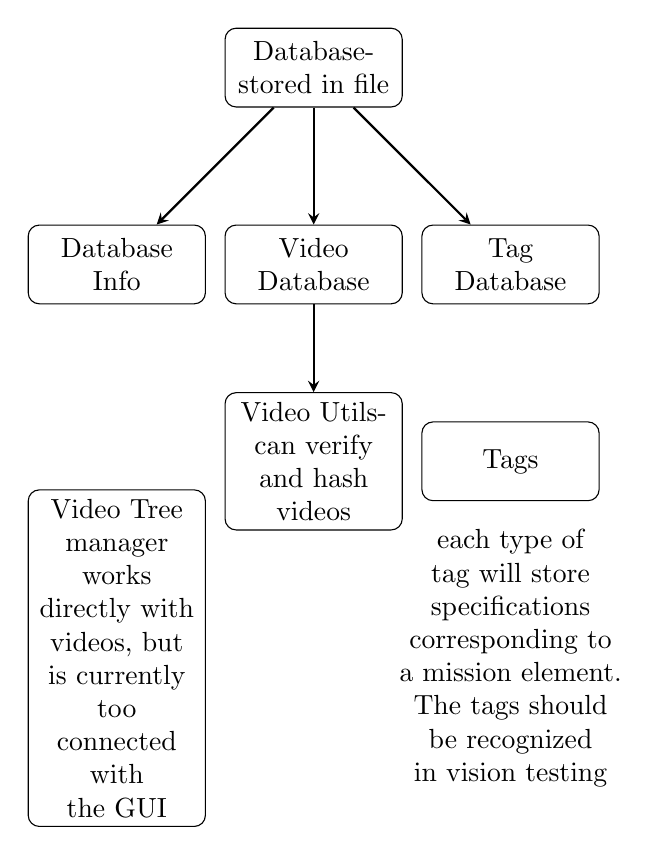
\begin{tikzpicture}[node distance=2.5 cm,scale =.5]

\node (database) [startstop] {Database-stored in file};
\node (vidD)[startstop ,below of =  database] {Video Database};
\node(vid) [startstop, below of= vidD] {Video Utils- can verify and hash videos};
\node (vidTree) [startstop, below of= vidD, left of=vid] {Video Tree manager works directly with videos, but is currently too connected with the GUI};
\node (tagD)[startstop ,right of = vidD] {Tag Database};
\node (dbInfo)[startstop ,left of = vidD] {Database Info};
\node (tag) [startstop, below of = tagD] {Tags};
\node (tagInfo)[clean, below of = tag] {each type of tag will store specifications corresponding to a mission element.  The tags should be recognized in vision testing};
% \node (test) [startstop, left of = vidD] {Video Testing};
% \node (testInfo) [clean, below of = test] {a vision algorithm should be ab};
\draw [arrow] (database) -- (dbInfo);
\draw [arrow] (database) -- (vidD);
\draw [arrow] (database) -- (tagD);
\draw[arrow](vidD)--(vid);
% \draw [arrow] (sb) -- (cs);
% \draw [arrow] (cs) -- (ef);


\end{tikzpicture}
% \includegraphics{}
\caption{CAVE functionality}
\label{fig:my_label}
\end{figure}
At the beginning of each season, new mission elements will need to be added to CAVE, to do this, open cave/libcave/mission\_elements.py and add a class of type MissionElement.  This file is how CAVE gets data from the shmlog files to work with testing, so please include all data that you want to compare and relative shm calls in this document.
\part{Test Functionality}
The original reason that CAVE was created was to help with vision algorithm tuning.  The testing that the GUI version performs leaves the user unclear as to how the resulting percentage is discovered.  To clear this up, the new version will have a variety of settings that the user can set for the test.  Such options should include the ability to return a list of the failed frames so the user can engage in thourough testing to figure out why the frames are failing.
\section{Process of Running a Test}
The user should be able to input the name of the vision algorithm to be run.  By default, the algorithm will run over all frames so that detection of other mission elements by this algorithm can be considered a false positive.  After the user specifies the video and the vision algorithm, the program should start visiond so that the user does not have to worry about whether or not the vision module has been started.  The testing code should make sure that the vision module is passed the cave\_test parameter.  Each frame of the video is passed to the vision system and is determined whether or not the test passed.  The user should be able to see what the test is accounting for, so they know how restrictive the constraints are.  Perhaps test constraints could be changed for each element.
\section{Measuring Accuracy}
The test should have a metric to determine whether or not a frame was successful.  We can compare data in the Shared Memory.  The test should tell the user which frames failed in addition to the frames that returned a false positive.
\section{Adding a Tag}

In the current cave system, to add a new tag to the database, the command calls the addTag class, which does not actually add a tag, it makes changes in the GUI, but then the tag is actually added in main.  To actually add a tag, the information needed is the tagName, missionElement, and tag\_type.  The call to add the tag to the database is Tag.tag\_new(name, missionElement, tag\_type).
\section{How To}
\subsection{Open a Database}
To perform further actions using CAVE, you first must load a database.
\begin{lstlisting}
auv-libcave load_db("database.cdb")
\end{lstlisting}

\subsection{Add a Video}
\begin{lstlisting}[breaklines=true]
auv-libcave addVideo("vidName", "Forward", "~/example.avi", "~/logs/log.shmlog")
\end{lstlisting}
or if you do not have the saved shmlog file,
\begin{lstlisting}
auv-libcave addVideo("video name", "Downward", "example.avi")
\end{lstlisting}
\subsection{Add Tag}
Adding a tag simply means that you are defining a way to recognize an object
\begin{lstlisting}[breaklines=true]
auv-libcave addTag("tagName", Pipe, center-visible)
\end{lstlisting}



\part{Conclusion}

This was a fun and educational semester for our subsubteam. We learned how to write both vision and mission modules as well as how to integrate the two into a complete mission. We are proud of our successful mission run during the semifinals of the mock competition.

Importantly, we were able to identify areas of the current software architecture upon which we might improve in the future, and became acquainted with development and debugging in a simulated competition environment.

We look forward to the future of our involvement with CUAUV!

\begin{flushright}
--- Victor Lucena, Jonathan Chan, and Page Bowers
\end{flushright}





\pagebreak



% Known Issues
\section{Known Issues}
The Video Tree Manager, which works directly with the Video database, is still connected with the GUI.  My nexts steps will be to separate these.

% current status
\section{Current Status}
The thruster board layout for the printed circuit board has been sent out. There were no known errors in schematic, layout, or gerbers. The printed circuit boards are expected to return on the last week of the semester. The thruster board will be populated and tested heavily in the beginning of the spring semester. Once one thruster board is completely populated, coded, and tested, the following thruster board will be equally populated in order to ensure motor control for all eight thrusters on the vehicle.


\pagebreak

% appendix



% datasheets




\end{document}

